Diese Zusammenfassung basiert zum grossen Teil auf der 100-Jahr Chronik, die 1974 von Walter Kaufmann-Lampart erstellt wurde.
\begin{figure}[ht]
    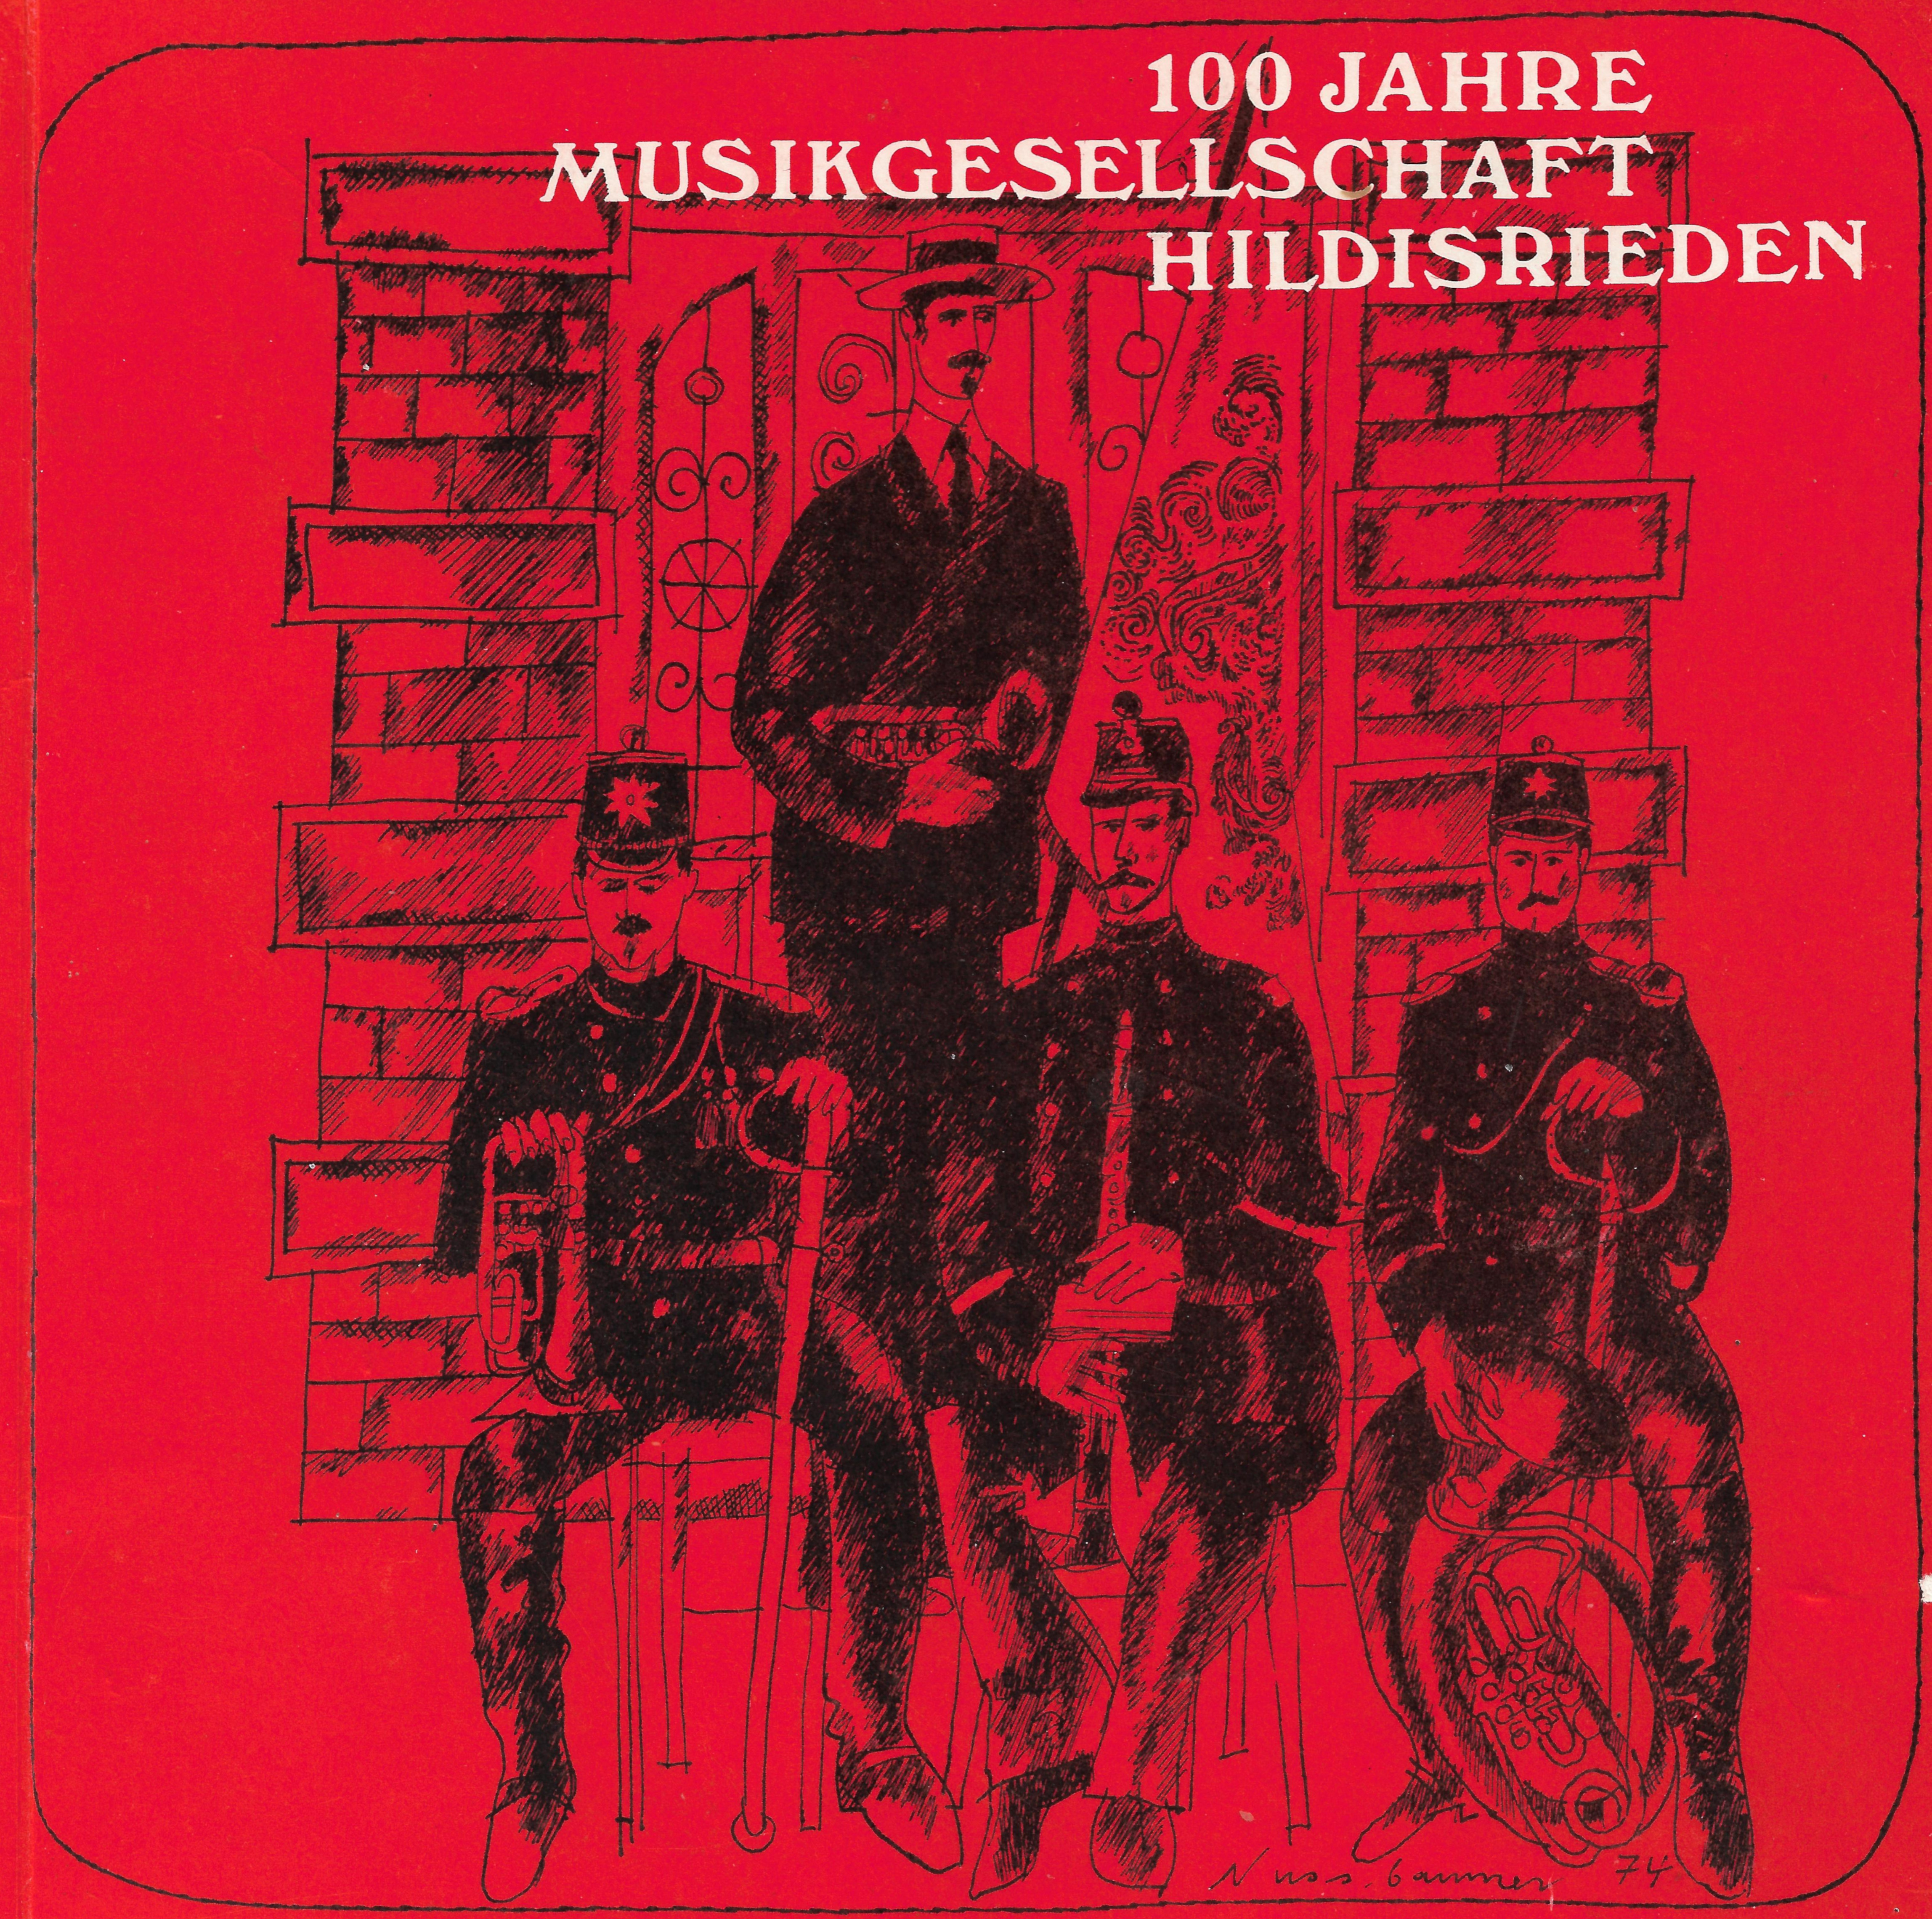
\includegraphics[scale=0.25]{./Cover-100-Jahr-Chronik.jpg}
\end{figure}
\subsection{Vorgeschichte}

\begin{history}

    Der 100. Geburtstag der Musikgesellschaft Hildisrieden gibt uns Gelegenheit,
    viel Wissenswertes und Heimatverbundenes über das musikalische Leben in
    unserem Dorfe zu erzählen. Die Verfassung dieser Erinnerungsschrift über die
    Geschichte und die Taten unserer Musikgesellschaft war keine leichte
    Aufgabe, weil das vorhandene Protokoll erst seit 1912 Auskunft gibt und
    alles vorher Geschehene von verschiedenen Seiten zusammengetragen werden
    musste.

    Dazu leisteten Veteranen und geschichtlich Interessierte wertvolle
    Dienste, was die Nachforschungen sehr erleichterte. Äusserst wertvolle
    Angaben über die Vorgeschichte der Blechmusik Hildisrieden machte uns Peter
    Muff, Lehrer, langjähriger Präsident und Dirigent, welcher alle
    Begebenheiten in ein Notizbuch niederschrieb.

    Diesem entnehmen wir, dass
    schon in den Jahren um 1860 Musikfreunde ein Blechquartett bildeten. Ihrer
    Tätigkeit nach zu schliessen muss angenommen werden, dass sie aus Liebe zur
    Musik und zum eigenen Vergnügen musizierten. In unserer Heimatgemeinde
    Hildisrieden, zwischen Sempacher- und Baldeggersee liegend, inmitten
    prächtiger Matten und Wiesen, wohl bestellter Äcker und gepflegter
    Obstgärten, ist eines erhalten geblieben, was damals schon unsere Ahnen für
    gut und recht fanden, nämlich die MUSIK.

    Musik in Freud und Leid, zu Tanz und Unterhaltung! So spielten sie an
    Weihnachten und Neujahr im Dorfe und auf den Gehöften von Schopfen,
    Traselingen, Holzmatt, Ohmenlingen und Oele.

    Musik ist eine dem Menschen von Natur aus angeborene Sache. Diese wurde im
    Laufe des Jahrhunderts in besonderem Masse in Hildisrieden gehegt und
    gepflegt. Bekanntlich vererben und erhalten sich Sitten und Bräuche in einem
    kleinen Dorfe von Generation zu Generation. So stellt man fest, dass die
    Familien Disler, Estermann und Troxler während drei Generationen das
    musikalische Leben in Hildisrieden prägten.

\end{history}
